\section{\texorpdfstring{Методы \mbox{классификации} с \mbox{использованием} \mbox{свёрточных} \mbox{нейронных} \mbox{сетей}}{Методы классификации с использованием свёрточных нейронных сетей}}
\textbf{Принцип работы свёрточных нейронных сетей}

Свёрточная нейронная сеть (Convolutional Neural Network, CNN) является типом модели глубокого обучения, предназначенной для обработки данных, имеющих решётчатую структуру, таких как изображения.

CNN представляет собой математическую модель, которая, как правило, состоит из трёх основных типов слоёв: свёрточных слоёв, слоёв подвыборки (pooling) и полносвязных слоёв. Свёрточные и pooling-слои используются для извлечения признаков, тогда как полносвязные слои выполняют отображение извлечённых признаков в выходные значения, например в классы при классификации изображений.

Свёрточный слой является ключевым компонентом архитектуры CNN и состоит из набора математических операций, включая свёртку~---~специализированный тип линейной операции. В цифровых изображениях значения пикселей хранятся в виде двумерной сетки чисел, и массив обучаемых параметров, называемый ядром, применяется ко всем локальным областям изображения. Благодаря этому CNN особенно эффективны для анализа изображений, поскольку один и тот же признак может появляться в различных частях изображения.

По мере прохождения данных через последовательные слои сети извлекаемые признаки становятся иерархически более сложными. Процесс настройки параметров сети, таких как ядра свёрточных слоёв и веса полносвязных слоёв, называется обучением и выполняется с целью минимизации различия между выходными предсказаниями сети и истинными метками обучающих данных.

В отличие от традиционных методов анализа изображений, где признаки извлекаются вручную, CNN позволяют автоматически извлекать признаки непосредственно из исходных изображений. Кроме того, архитектуры CNN, как правило, не требуют предварительной сегментации объектов, выполняемой экспертами, что снижает зависимость качества модели от субъективных факторов. Однако CNN содержат большое количество обучаемых параметров, что требует значительных вычислительных ресурсов и наличия достаточно больших наборов обучающих данных. Для эффективного обучения CNN обычно используются графические процессоры (GPU).

Архитектура CNN включает свёрточные слои, pooling-слои и полносвязные слои. Типичная архитектура состоит из повторяющихся блоков, включающих один или несколько свёрточных слоёв и слой подвыборки, за которыми следуют полносвязные слои. Процесс преобразования входных данных в выходные значения посредством последовательного прохождения через слои сети называется прямым распространением (forward propagation).

\textbf{Свёрточный слой}


Свёрточный слой выполняет извлечение признаков и является фундаментальным элементом CNN. Он состоит из линейной операции свёртки, за которой следует нелинейная функция активации.

\textbf{Операция свёртки}


Свёртка представляет собой специализированный тип линейной операции, при которой массив чисел, называемый ядром, применяется к входному тензору. В каждой позиции выполняется поэлементное произведение элементов ядра и соответствующих элементов входного тензора, результаты которого суммируются для получения значения в выходной карте признаков.

Применение нескольких ядер позволяет формировать несколько карт признаков, каждая из которых отражает различные характеристики входных данных. Таким образом, различные ядра могут рассматриваться как отдельные извлекатели признаков.

Основными гиперпараметрами операции свёртки являются размер ядра и их количество, что определяет глубину выходных карт признаков.

Поскольку стандартная операция свёртки приводит к уменьшению пространственных размеров выходного тензора, часто применяется метод дополнения, при котором по краям входного тензора добавляются нулевые значения. Это позволяет сохранить пространственные размеры карт признаков.

Ключевой особенностью операции свёртки является совместное использование весов, при котором одно и то же ядро применяется ко всем позициям изображения. Это обеспечивает инвариантность к сдвигу, формирование иерархий признаков и уменьшение числа обучаемых параметров по сравнению с полносвязными сетями.

\textbf{Функция активации}


После линейной операции свёртки применяется нелинейная функция активации. В современных CNN наиболее распространённой функцией активации является выпрямленная линейная единица (Rectified Linear Unit, ReLU), определяемая как $\max(0, x)$.

\textbf{Pooling-слой}


Pooling-слой используется для понижения пространственной размерности карт признаков и повышения устойчивости модели к небольшим сдвигам и искажениям. В pooling-слоях отсутствуют обучаемые параметры, однако размер фильтра, шаг и способ подвыборки задаются как гиперпараметры.

\textbf{Max-pooling}


Max-pooling является наиболее распространённой pooling-операцией, при которой из каждого локального фрагмента карты признаков выбирается максимальное значение. Обычно используется фильтр размером $2 \times 2$ с шагом 2, что уменьшает высоту и ширину карты признаков в два раза.

\textbf{Глобальный average-pooling}


Глобальный average-pooling преобразует карту признаков в тензор размером $1 \times 1$ путём усреднения всех значений. Эта операция позволяет уменьшить количество параметров модели и обеспечивает возможность обработки входных изображений переменного размера.

\textbf{Полносвязные слои}


Выходные карты признаков последнего свёрточного или pooling-слоя преобразуются в одномерный вектор и подаются на вход одного или нескольких полносвязных слоёв. Эти слои выполняют отображение извлечённых признаков в выходное пространство, например в вероятности классов.

Для задач многоклассовой классификации в последнем слое обычно используется функция активации softmax, которая нормализует выходные значения в вероятности, сумма которых равна единице.

\textbf{Обучение и функция потерь}


Обучение CNN заключается в настройке параметров сети~---~ядер свёрточных слоёв и весов полносвязных слоёв~---~таким образом, чтобы минимизировать функцию потерь, измеряющую расхождение между предсказаниями сети и истинными метками обучающих данных.

Функция потерь выбирается в зависимости от решаемой задачи. Для задач классификации обычно используется перекрёстная энтропия, тогда как для задач регрессии применяется среднеквадратичная ошибка.

Градиентный спуск обычно используется в качестве алгоритма оптимизации, который итеративно обновляет обучаемые параметры сети, то есть ядра и веса, с целью минимизации функции потерь.

\textbf{Примеры моделей CNN}

\textbf{AlexNet}

Архитектура AlexNet была предложена Алексом Крижевским и Джеффри Хинтоном. Архитектура сети, использованная в данной работе, представлена на рис.~\ref{arch_alex}. Сеть AlexNet содержит восемь взвешенных слоёв, первые пять из которых являются свёрточными слоями, а оставшиеся три~---~полностью связанными слоями.

За первыми двумя свёрточными слоями следуют слои нормализации и пулинга. После последнего свёрточного слоя располагается один слой пулинга. Третий, четвёртый и пятый свёрточные слои соединены напрямую. Второй полностью связанный слой передаёт данные классификатору softmax, который формирует вероятности принадлежности к классам.

В качестве функции активации в первых двух полностью связанных слоях (fc6 и fc7) используется функция ReLU, которая генерирует 4096 значений. Выход седьмого слоя, содержащий 4096 элементов, полностью соединён с нейронами восьмого слоя (fc8), где число нейронов соответствует количеству классов. После обучения выходной слой fc8 формирует значения с плавающей запятой, представляющие прогнозируемый результат классификации.

\begin{figure}[h]
	\centering
	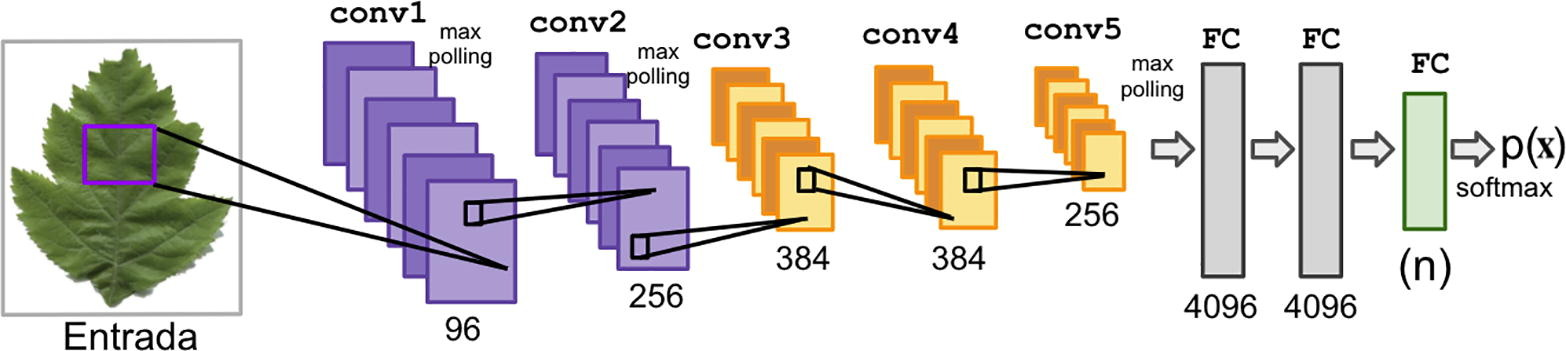
\includegraphics[width=\linewidth]{inc/img/arch_alex.jpg}
	\caption{Архитектура AlexNet}
	\label{arch_alex}
\end{figure}

\textbf{GoogLeNet}


Архитектура GoogLeNet стала победителем конкурса ILSVRC 2014 года, продемонстрировав ошибку 6{,}67\% по метрике top-5. Данная архитектура показала высокую эффективность при решении задач, характеризующихся высокой сложностью, достигнув высокой точности при относительно низкой вычислительной нагрузке.

В отличие от AlexNet, GoogLeNet реализует иной подход к построению сети и включает в себя специализированные структурные элементы, называемые модулями inception. Общая структура архитектуры GoogLeNet представлена на рис.~\ref{arch_google}. Модуль inception использует переменные рецептивные поля, сформированные с помощью свёрточных ядер различного размера. Это позволяет эффективно фиксировать редкие корреляционные паттерны в картах признаков.

Архитектура GoogLeNet состоит из 22 слоёв, что существенно превышало глубину ранее предложенных сетей. При этом количество параметров в GoogLeNet значительно меньше и составляет примерно одну двенадцатую от числа параметров AlexNet. В архитектуре используются девять модулей inception (M1--M9). Основная идея inception заключается в локализации оптимальной разреженной структуры и её аппроксимации плотным представлением.

Каждый модуль inception включает несколько свёрток с ядрами размером $1\times1$, $3\times3$ и $5\times5$, а также слой max-pooling, результаты которых объединяются. Такой подход отличает GoogLeNet от традиционной многоканальной свёртки. Для снижения вычислительной сложности и предотвращения переобучения применяются стратегии усредняющего пулинга и отсева после модулей inception, что способствует уменьшению размерности признакового пространства. Более подробное описание данной архитектуры приведено в~\cite{ref40}.

\begin{figure}[h]
	\centering
	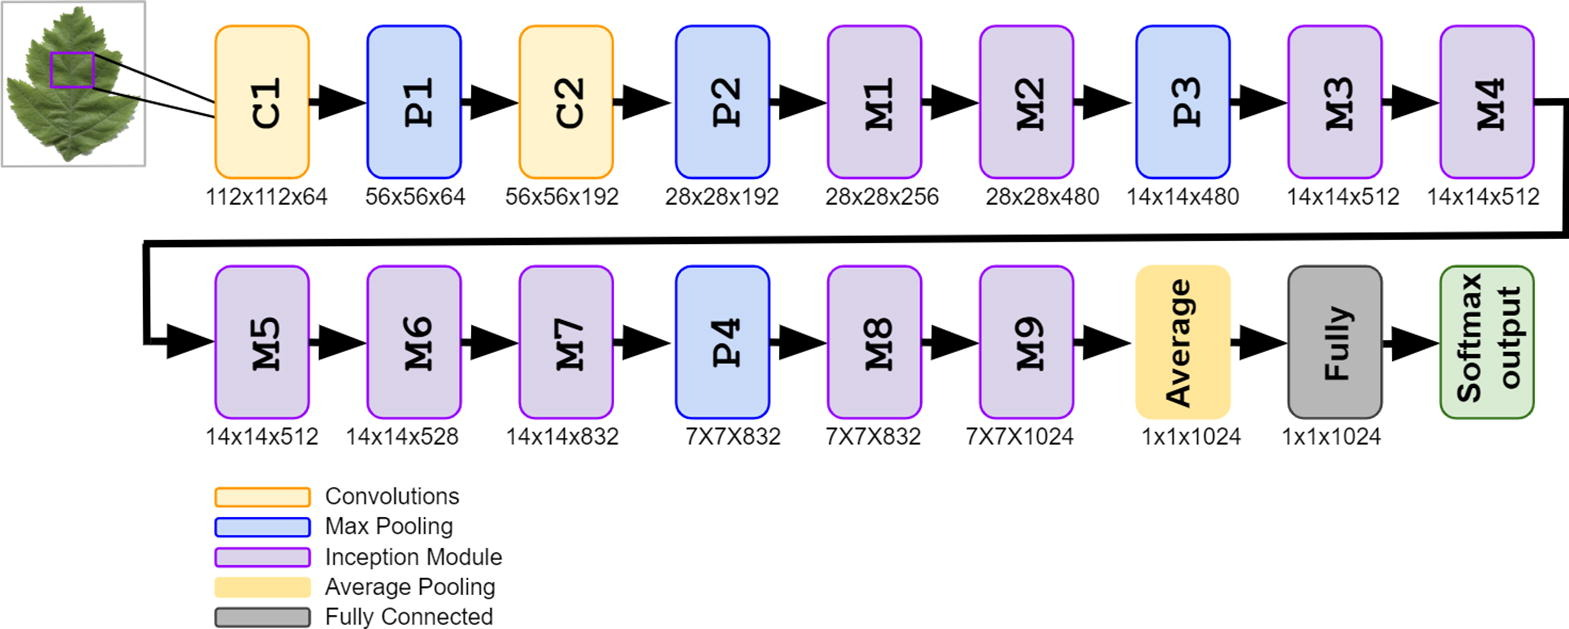
\includegraphics[width=\linewidth]{inc/img/arch_google.jpg}
	\caption{Архитектура GoogLeNet}
	\label{arch_google}
\end{figure}

\textbf{VGGNet}


Архитектура VGGNet была разработана Кареном Симоняном и Эндрю Зиссерманом и заняла второе место в конкурсе ILSVRC 2014 года. VGGNet представляет собой развитие идей, заложенных в архитектуре AlexNet. Структура сети показана на рис.~\ref{arch_vgg}.

Основной особенностью VGGNet является использование исключительно свёрточных ядер размером $3\times3$ и слоёв максимального пулинга размером $2\times2$. Архитектура VGG включает пять блоков свёрточных слоёв, каждый из которых завершается слоем максимального пулинга. После свёрточных блоков следуют два полностью связанных слоя и выходной слой.

Первые два блока содержат по два свёрточных слоя с 64 и 128 фильтрами соответственно. Следующие два блока включают по три свёрточных слоя с 256, 512 и 512 фильтрами. Все слои максимального пулинга имеют размер окна $2\times2$ и шаг, равный 2.

VGGNet является одной из наиболее популярных архитектур в литературе для извлечения признаков из изображений. Однако данная архитектура содержит около 138 миллионов параметров, что может затруднять её практическое использование. В литературе широко представлены модификации VGGNet, такие как VGG16 и VGG19. В данной работе использовалась архитектура VGG16, состоящая из 16 глубоких свёрточных слоёв.

\begin{figure}[h]
	\centering
	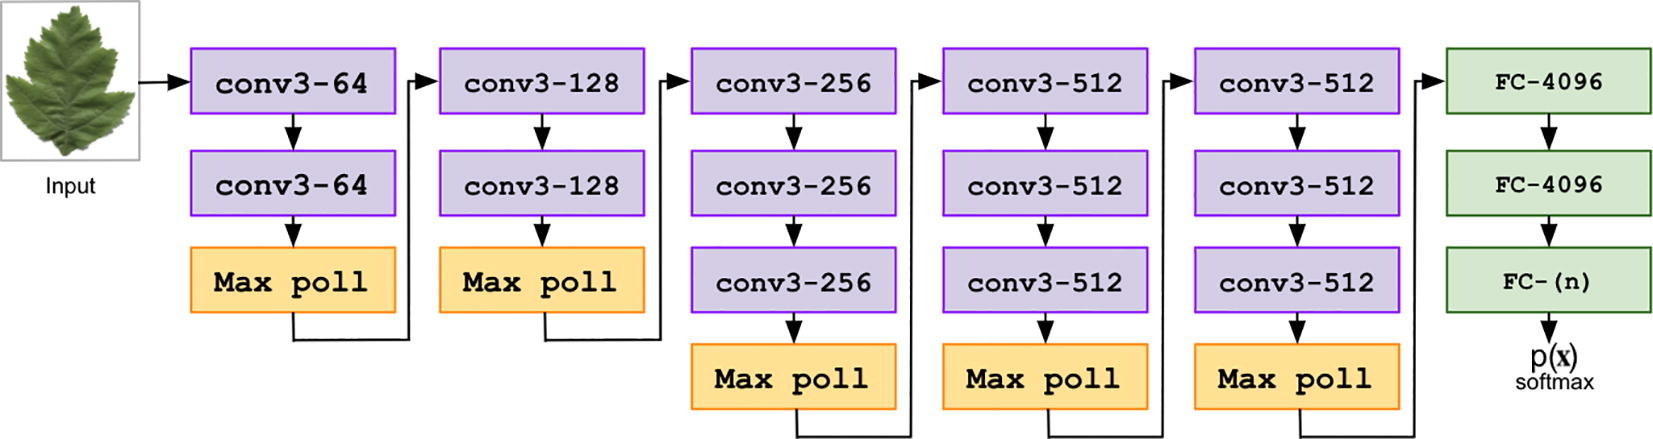
\includegraphics[width=\linewidth]{inc/img/arch_vgg.jpg}
	\caption{Архитектура VGGNet}
	\label{arch_vgg}
\end{figure}
\textbf{FGIC-классификация}

В методах FGIC (fine-grained image classification) распознавание проводится по иерархии классов. Для растений такая иерархия естественным образом задаётся ботанической таксономией, включающей уровни семейства, рода и вида. Эксперты-ботаники традиционно используют именно такой подход, определяя род растения и уточняя конкретный вид~\cite{ref35}. 

Иерархический подход снижает сложность классификации за счёт поэтапного уточнения решения: на первом этапе производится грубая классификация по более общим таксономическим категориям, после чего выполняется детальная классификация внутри ограниченного подмножества классов. Такой подход позволяет сгруппировать визуально схожие объекты и тем самым уменьшить влияние межклассовых и внутриклассовых вариаций.

Различия между близкими видами характеризуются низкой вариативностью формы и цвета, поэтому при детальной классификации используется локальное представление изображения листа.

\textbf{Сиамские нейронные сети}

Сиамские нейронные сети (SCNN) представляют собой нейронные сети, состоящие из двух или более симметричных (идентичных) подсетей. Ключевым признаком, позволяющим отнести сеть к классу сиамских, является совместное использование весов между идентичными подсетями~\cite{ref78}. Сиамская сеть функционирует следующим образом: входные данные подаются параллельно во все идентичные подсети, после чего производится сравнение выходных представлений, и на основе этого сравнения принимается решение о принадлежности входных данных (изображения) к тому или иному классу~\cite{ref79}.

SCNN имеет схожую структуру с CNN, включая свёрточные и pooling-слои, однако в ней отсутствует слой softmax. В отличие от обычных CNN, разность выходов полносвязных слоёв передаётся на один нейрон с монотонной функцией активации (чаще всего сигмоидной), формирующей бинарный выход (0 или 1). Общая архитектура сиамской нейронной сети показана на рис.~\ref{scnn_example}

\begin{figure}[h]
	\centering
	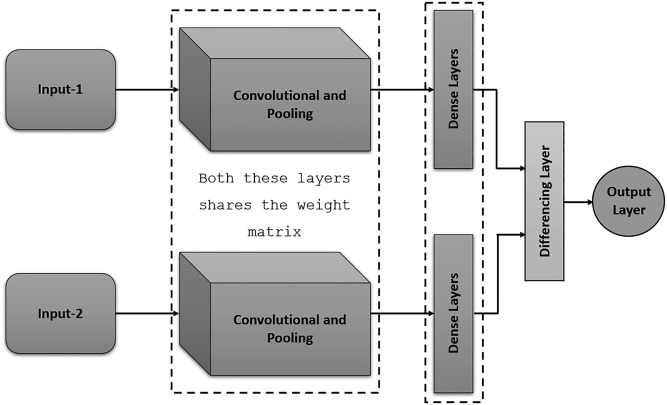
\includegraphics[width=\linewidth]{inc/img/SCNN_example.jpg}
	\caption{Архитектура SCNN}
	\label{scnn_example}
\end{figure}
\textbf{Гибридные подходы}

В работе "On the Behavior of Convolutional Nets for Feature Extraction"~\cite{ref1006} показано, что обученные CNN способны извлекать визуальные дескрипторы, которые можно использовать в задачах, отличных от исходной задачи обучения сети, без необходимости дорогостоящей фазы обучения на целевых данных. Применение такого подхода обычно заключается в извлечении признаков из слоёв сети, близких к выходу, и последующей подаче этих признаков в классический классификатор, что обеспечивает устойчивую и информативную характеристику изображений~\cite{ref1006}. Извлечённые признаки могут использоваться в других задачах машинного обучения, включая классификацию, кластеризацию или оценку сходства, без повторного обучения самой сети.

В работе "Two-view fine-grained classification of plant species"~\cite{ref1007} авторы предлагают использование иерархического подхода с глобальным и локальным представлением листа, используя SCNN в качестве основной архитектуры, поскольку одной из главных задач является классификация визуально схожих видов общего рода при малом количестве данных. Благодаря использованию SCNN не требуется переобучения при добавлении новых видов, поскольку результатом работы является не класс, а сходство между тестовым и эталонными изображениями. Предложенный подход иллюстрируется на рис.~\ref{super_example}.

\begin{figure}[h]
	\centering
	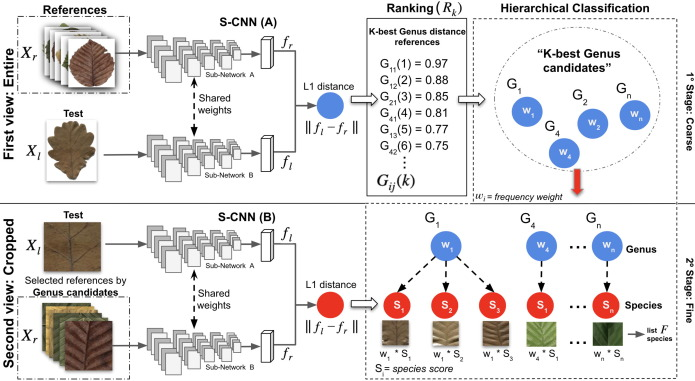
\includegraphics[width=\linewidth]{inc/img/super_example.jpg}
	\caption{Иерархическая классификация с использованием SCNN}
	\label{super_example}
\end{figure}

\section{Сравнительный анализ подходов}

Для анализа применимости рассмотренных подходов к задаче тонкозернистой классификации изображений растений вводится совокупность критериев, охватывающих как количественные характеристики качества классификации, так и концептуальные свойства методов.

Введены следующие критерии сравнения:
\begin{enumerate}
	\item тип используемых признаков;
	\item требуется ли повторное обучение при добавлении новых классов;
	\item зависимость качества от объёма размеченных данных;
	\item вычислительная сложность обучения;
	\item вычислительная сложность инференса;
	\item интерпретируемость используемых признаков;
	\item применимость к задачам тонкозернистой классификации изображений.
\end{enumerate}

На основе введённых критериев составлена сравнительная таблица~\ref{criteries_table}, позволяющая проанализировать сильные и слабые стороны рассмотренных подходов в контексте задачи классификации изображений растений.

\begin{table}[h]
	\centering
	\caption{Сравнение подходов к классификации изображений растений по строгим критериям}
	\label{criteries_table}
	\renewcommand{\arraystretch}{1.2}
	\resizebox{\linewidth}{!}{%
		\begin{tabular}{|p{5.2cm}|c|c|c|c|c|}
			\hline
			\textbf{Критерий / подход} & \textbf{\begin{tabular}[c]{@{}c@{}}LBP/HOG\\+ kNN/SVM\end{tabular}} & \textbf{\begin{tabular}[c]{@{}c@{}}CNN\\end-to-end\end{tabular}} & \textbf{\begin{tabular}[c]{@{}c@{}}CNN как\\экстрактор\end{tabular}} & \textbf{\begin{tabular}[c]{@{}c@{}}Siamese\\CNN\end{tabular}} & \textbf{\begin{tabular}[c]{@{}c@{}}Комбинированный\\\end{tabular}} \\
			\hline
			Тип признаков & ручные & обучаемые & обучаемые & обучаемые & обучаемые \\
			\hline
			Требуется повторное обучение при добавлении новых классов & нет$^{*}$ & да & нет$^{**}$ & нет$^{**}$ & нет$^{**}$ \\
			\hline
			Зависимость качества от объёма размеченных данных & высокая & высокая & средняя & ниже & ниже \\
			\hline
			Вычислительная сложность обучения & низкая & высокая & низкая--средняя & высокая & высокая \\
			\hline
			Вычислительная сложность инференса & низкая & средняя & средняя & высокая & высокая \\
			\hline
			Интерпретируемость используемых признаков & высокая & низкая & низкая & низкая & низкая \\
			\hline
			Типичная область применимости в FGIC & ограниченно & да & да & да & да \\
			\hline
	\end{tabular}}
	\vspace{2mm}
	
	{\footnotesize $^{*}$ Добавление нового класса возможно без переобучения при условии переразметки/донастройки классификатора и наличия признаков для новых образцов. \\
		$^{**}$ Добавление нового класса возможно путём добавления эталонных образцов (reference images) без изменения весов модели при метрической постановке задачи.}
\end{table}
